\chapter{АНАЛІЗ ПРЕДМЕТНОЇ ОБЛАСТІ І ПОСТАНОВКА ЗАДАЧІ}

\section{Постановка задачі}
Поставимо такий набір задач для нашого додатку:
\begin{enumerate}
\item Користувач може спілкуватись з чат-ботом у одному з існуючих месенджерів.
\item Бот має кілька готових простих реплік на різні ситуації.
\item Бот вміє розпізнавати тип повідомлення.
\item Бот вміє робити нагадування.
\item Бот вміє дізнаватися просту інформацію з сторонніх сервісів.
\item Бот може розпізнавати деякі теми у повідомленні
\item Бот може розпізнавати іменовані сутності.
\item Бот може розпізнавати загальний тон повідомлення.
\item Бот може відповідати на деякі прості питання по інформації, що надав йому користувач.
\item Бот зберігає інформацію про користувача.
\item Бот генерує датасети для майбутнього покращення роботи бота.
\item Бот відповідає на повідомлення у прийнятний час - не більш, ніж 5 секунд.
\end{enumerate}


Такий набір завдань гарантує можливість використовувати бота як простого асистента. Крім того, враховуючи зберігання інформації про користувача та можливість відповідати на питання про нього, ми можемо покращити внутрішню роботу бота - наприклад, якщо бот знає відповідь на питання "Де проживає користувач"  то бот може пропонувати користувачу сценарії та повідомлення, враховуючи дану інформацію.
\newpage


\section{Огляд існуючих рішень серед схожих застосунків}
Через стрімкий розвиток технологій, пов'язаних з обробкою та генерацією природньої мови, все більшу і більшу популярність у світі набирають чат-боти. Цей вибух популярності підтримується в тому числі бізнесами, яким необхідно спростити комунікацію з клієнтами та відсікти якомога більше простих запитань та взаємодій з користувачами, щоб не перевантажувати живих працівників та зменшити час очікування відповіді. Крім того, завдяки існуючим технологіям та фреймворкам, що дозволяють ніби з цеглинок будувати нових чат-ботів, вартість розробки та підтримки таких чат-ботів стає дешевшою, ніж розширення команди технічної підтримки. Також однією з переваг чат-ботів є те, що за тим, як користувачі користуються ними та як реагують на різні сценарії, простіше будувати аналітику та приймати рішенння щодо майбутнього розвитку бізнесу.


Є також і інший аспект розвитку чат-ботів - так звані персональні асистенти. У даному випадку вони використовуються компаніями не для підтримки своїх основних продуктів, а як окрема програма, яка спрощує життя користувачеві та допомагає йому з деякими рутинними задачами. Серед найвідоміших персональних асистентів - чат-боти від Apple. Google, Amazon та Microsoft. 


Для таких великих компаній розробка персональних асистентів є значно спрощеною, тому що вони можуть запропонувати просту інтеграцію з власними сервісами компаній - наприклад Google Assistant має доступ до календаря користувача, його електронної пошти, тощо. Також великі компанії такого розміру активно фінансують дослідження у сфері роботи з природньою мовою, що дає їм можливість користуватися кращими моделями та мати до них доступ раніше за інших. Ще одніює перевагою цих компаній є те, що в них значно більше даних, що допомагає натреновувати значно кращі моделі.
\subsection{Siri}
Siri [1] - один із найперших та найвідоміших персональних асистентів, що був представлений для пристроїв на iOS ще у 2010 році. Однією з перших його функцій було розпізнавання голосу та простих запитів від користувачів. З тих пір, персональний асистент постійно оновлюється, а його функціональність розширюється. Важливою перевагою Siri є глибока інтеграція з усіма сервісами Apple, що  гарно лягає у ідею єдиної екосистеми.
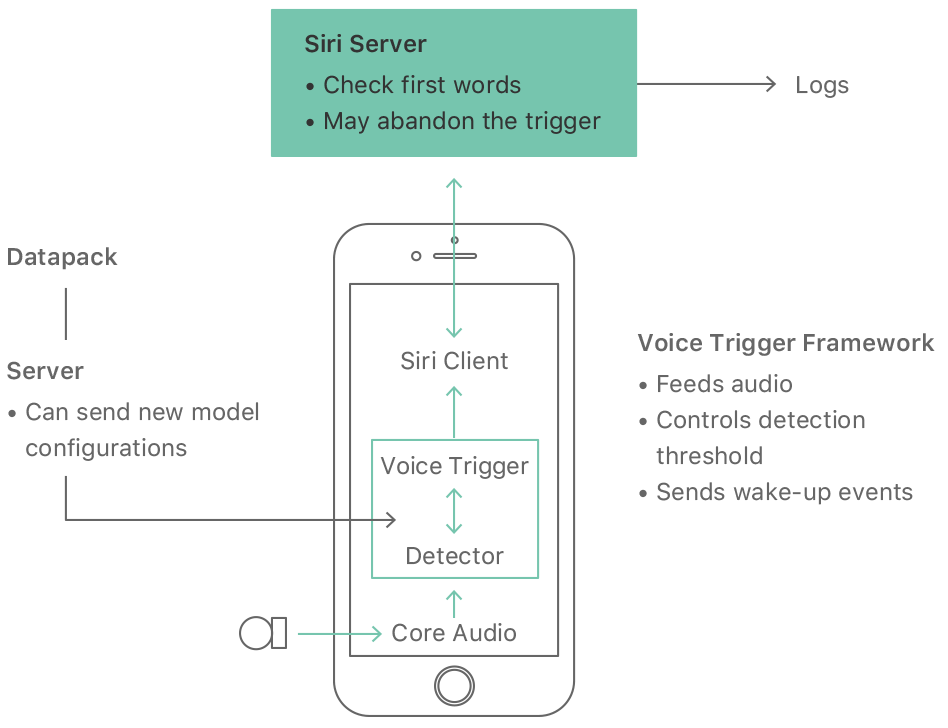
\includegraphics[width = 500]{Dissertation/siri.png}\\
\textit{рис 1. Приклад обробки запиту "Hey, Siri"}


Важливість Siri полягає у тому, що на час запуску технології розпізнавання голосу та розпізнавання мови не були настільки пошиерні, тому, Siri є в певному сенсі першопрохідцем на ринку персональних асистентів.

З іншого боку, її суттєвим недоліком є те, що її функціонал значно обмежений з двох причин. Першою є те, що Siri обмежена тими пристроями, на яких вона запускається - у більшості своїй це телефони та планшети, а не домашні колонки як у конкурентів. Окрім цього, Apple не надає доступу стороннім розробникам доступу до API Siri, через що вона має значно менше функцій, ніж наприклад Alexa.



\subsection{Google Assistant}
Google Assistant[2] - персональний асистент від компанії Google. По суті, це окрема програма, у якій користувач може спілкуватись текстом з асистентом, але Google також випускає асистента у вигляді окремої звукової колонки Google Home разом з озвучкою асистенту та здатністю сприймати голос користувача. 

Серед основних переваг асистента - інтеграція з усіма сервісами Google, що дає змогу поєднувати багато задач у одному асистенті. Крім того, Google Home вміє розпізнавати різні голоси користувачів, що дає можливість персоналізувати взаємодію з ботом навіть у випадку якщо декілька користувачів користуються одним і тим ж е самим пристроєм.

Асистент може робити все на чому спеціалізується Google - шукати на картах, повідомляти останні новини, знаходити інформацію у пошуковики, вмикати музику з Google Music. Також, для створення більш приємного враження від взаємодії з асистентом, у ньому закладено багато сценаріїв та відповідей накшталт "пожартуй" або "розкажи мені казку".

Колонка Google Home також вміє інтегруватись з оточуючими пристроями, такими як датчики та прибори розумного дому, розумні телевізори (через Google Chromecast), тощо.
\subsection{Amazon Alexa}
Amazon Alexa[3] - персональний асистент, інтегрований у аудіопристрої від компанії Amazon. Як і у випадку з Google Assistant, асистент заточений під сервіси компанії, що його розробляє, але бот має і багато інших функцій, серед яких стандартні погода, календар, нагадування, тощо. 

Однією з переваг Alexa є так звані Alexa Skills - Amazon надає API для розробки власних функцій бота, які можна публікувати у спеціальному маркетплейсі. Після цього, будь-який користувач може включити нову функціональність для себе. 

Amazon Lex[4] - технологія розпізнавання мовлення і обробки природньої мови, на основі якої побудована Alexa, є відкритою для розробників. Вони можуть будувати своїх чат-ботів на основі цієї технології.
\section{Огляд існуючих моделей для розв'язування задач}
\subsection{Question-answering моделі}
У 2016 році в [5] було представлено датасет, що складається з 100000 питань з можливими варіантами правильних відповідей по більше, ніж 500 статтям з Вікіпедії. У 2018 році в [6] було оновлено датасет, до нього було додано запитання, що не мають відповіді. 
У 2018 році в [7] було запропоновано модель BERT, що серед інших відомих задач показала два state-of-the-art результати для SQuAD v2.0 і SQuAD v1.1. Наразі, найкращі результати на даних датасетах показують моделі, похідні від BERT - або його модифікації, або використання його у ансамблі з іншими потужними моделями. 
\subsection{Sentiment-analysis моделі}
Є два відомих датасети для оцінювання моделей, призначених визначати тон повідомлення. Першим є збірник відгуків на кінофільми на сайті IMDB, представлений у [8], що складається з 50000 відгуків.  Другим є анотований збірник твітів, що був представлений у [9] та складається з 1,6 міліонів повідомлень з оцінкою тону.
\subsection{Named entity recognition}
Проблема розпізнавання іменованих сутностей є класичною задачею у сфері обробки природньої мови. Вона полягає у знаходженні у тексті власних назв та розпізнавання того, що саме описує власна назва - людину, місце, тощо. \\
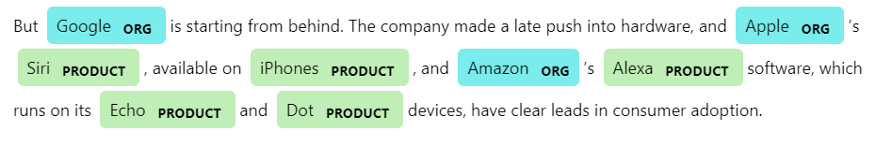
\includegraphics[width = 500]{Dissertation/ner-example.png}\\
\textit{рис 2. Приклад розпізнавання іменованих сутностей.}


У розв'язанні цієї задачі використовуються наступні підходи[10]:
\begin{enumerate}
\item Класичний rule-based підхід.
\item Підходи, що базуються на машинному навчанні.
\item Підходи, що базуються на глибокому навчанні.
\item Комбінації машинного і глибокого навчання. 
\end{enumerate}
Датасетом для перевірки моделей є CoNLL-2003, описаний у [11]. Однією з моделей, що показують state-of-the-art результат, є модель NER DL Annotator [12], представлена у вільнопоширюваній бібліотеці Spark NLP.
\subsection{Spark NLP}
Spark NLP[13] - вільнопоширюванна бібліотека для роботи з природніми мовами. Основною її частиною є натреновані моделі, що мають назву анотатори. Ці моделі можна калібрувати на власних даних та використовувати у так званих пайплайнах.\\
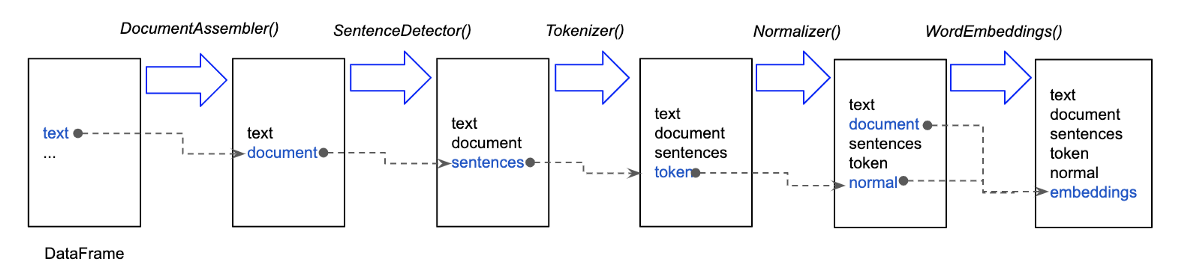
\includegraphics[width = 450]{Dissertation/spark_nlp.png}\\
\textit{рис 3. Демонстрація роботи пайплайну}

Пайплайн - набір моделей, трансформерів та оцінювачів (естіматорів), що послідовно застосовуються до вхідних даних. Spark NLP має кілька заздалегідь натренованих пайплайнів, що маю високі результати у типових задачах обробки природньої мови. 

Для виконання задачі word embeddings, бібліотека використовує натреновану модель BERT, що дає можливість значно покращити результати.

Бібліотека працює на основі двох інших відомих бібліотек - Apache Spark і Apache Spark ML. Оскільки вони підтримуються для мов програмування Scala, Java і Python, то і бібліотека Spark NLP підтримується для усіх цих мов. 

Spark NLP має моделі, натреновані для різних мов, серед яких англійська, французька, італьянська, тощо.
